\documentclass[12pt,a4paper]{article}

\usepackage[margin=1in]{geometry}
\usepackage{graphicx}
\usepackage{amsmath}
\usepackage{booktabs}
\usepackage{array}
\usepackage{float}
\usepackage{setspace}
\usepackage{hyperref}

\setstretch{1.12}
\setlength{\parindent}{0pt}
\setlength{\parskip}{0.5em}
\hypersetup{colorlinks=true,linkcolor=black,urlcolor=blue,citecolor=black}

\title{\textbf{Simulation-Based Implementation of Lean Manufacturing Techniques for Productivity Improvement:}\\
\textbf{A Data-Driven Case Study From a Beverage Bottling Line}}
\author{
Divash Krishnam \and Ashutosh Verma \and Raja \\
\small Department of Production and Industrial Engineering \\
\small Guided by Dr.\ MOHD SHUAIB, Mechanical Department
}
\date{March 26, 2026}

\begin{document}

\maketitle

\begin{abstract}
Lean manufacturing is widely recognized as an effective strategy for improving productivity, reducing waste, and stabilizing production flow. However, many small and medium-sized manufacturing firms still face difficulty in deciding which lean techniques should be implemented first, especially when resources are limited and repeated experimentation on the shop floor is risky. This paper develops a self-contained, data-driven framework for evaluating lean interventions using a real industrial production dataset from a beverage bottling line monitored through an Industrial Internet of Things system. The dataset contains 59 production summary records across 56 calendar production days between July 22, 2022 and February 6, 2023, 265 hourly operating observations, and 1,388 downtime events. The production system is analyzed through throughput, operating time, pause time, product mix, and temporal efficiency variation. Downtime events are then classified into micro-, minor-, and major-stoppage categories to identify the dominant source of waste. Finally, an event-level bootstrap simulation with 5,000 replications is used to compare three lean scenarios: 5S with visual management, total productive maintenance, and an integrated lean bundle. The observed system produced 212,358 liters with an overall availability of 42.66\%. Downtime analysis shows that micro-stoppages represent 61.31\% of all events but only 13.59\% of downtime minutes, whereas major stoppages represent only 6.77\% of events but consume 66.26\% of lost time. Simulation results show that 5S and visual management improve output by 2.33\%, total productive maintenance improves output by 20.61\%, and the integrated lean bundle improves output by 32.19\%, while increasing simulated availability from 42.37\% to 55.33\%. The study concludes that maintenance-led reduction of major stoppages should be prioritized before broader workplace-stabilization measures when downtime severity is highly concentrated.
\end{abstract}

\textbf{Keywords:} Lean manufacturing, productivity improvement, discrete-event simulation, downtime analysis, bottling line, total productive maintenance, 5S, IIoT, SMEs.

\section{Introduction}
Lean manufacturing has remained one of the most influential improvement philosophies in industrial engineering because it aims to eliminate non-value-added activity while improving flow, quality, and responsiveness. In production systems with unstable operation, the practical challenge is not whether lean is useful, but which lean technique should be prioritized first. This challenge becomes more serious for SMEs and small-scale operations, where technical staff, budgets, and improvement time are limited. A wrong implementation sequence can consume management attention without delivering meaningful productivity gains.

Simulation is valuable in this context because it enables organizations to test lean interventions before changing the actual production system. Several prior studies have shown that lean practices improve operational performance, but the size of that improvement depends on the manufacturing context [1], [4], [5]. More recent work also shows that lean manufacturing and digital manufacturing increasingly reinforce one another because real operational data improve diagnosis and improvement selection [6], [10].

This paper addresses that opportunity by using an open industrial dataset from a beverage bottling line [8]. The dataset is particularly useful because it combines production summaries, hourly operating information, and detailed downtime-event logs gathered through an IIoT-based monitoring system [7]. Using these data, the present study develops a reproducible simulation-based evaluation of lean alternatives.

The objectives of the study are:
\begin{enumerate}
    \item to analyze the production and downtime behavior of the bottling line;
    \item to identify the dominant operational waste pattern;
    \item to simulate the impact of selected lean interventions on productivity; and
    \item to recommend a practical implementation priority for lean techniques.
\end{enumerate}

\section{Literature Review and Research Gap}
Belekoukias \emph{et al.} [1] showed that lean tools can improve operational performance, but they also highlighted that the magnitude of improvement depends strongly on context. Oleghe and Salonitis [2] argued that lean systems still require stronger quantitative modeling, especially where process variability and human interaction influence production behavior.

Simulation has increasingly become a preferred method for evaluating lean choices. Yu and Chen [3] reviewed factory simulation in SMEs and concluded that simulation is useful but still underutilized because SMEs need more practical and transferable applications. Possik \emph{et al.} [4] proposed a co-simulation framework for evaluating lean techniques and showed that different tools have different leverage depending on system structure. Frecassetti \emph{et al.} [5] demonstrated that simulation can support the introduction of lean practices in an SME by comparing interventions before implementation.

The literature also shows a growing convergence between lean and digital manufacturing. Bokhorst \emph{et al.} [6] found that smart manufacturing often builds on lean principles. Reslan \emph{et al.} [10] further showed that digital twins can strengthen value stream mapping and lean diagnosis. In food and beverage SMEs, Matindana and Shoshiwa [9] found that lean implementation is highly relevant, but event-level data-driven case studies remain limited.

The main research gap is therefore clear: many lean-simulation studies remain proprietary, difficult to reproduce, and disconnected from open event-level production data. This paper addresses that gap by integrating real downtime-event data, lean scenario design, and simulation-based productivity analysis in a reusable academic case.

\section{Problem Formulation}
The main problem studied here is to determine which lean intervention should be given priority when a production line experiences both frequent short interruptions and a small number of severe stoppages.

The key relationships used in the analysis are:
\begin{equation}
A = \frac{T_{op}}{T_{mon}}
\end{equation}
\begin{equation}
T_{dt} = T_{mon} - T_{op}
\end{equation}
\begin{equation}
R = \frac{Q}{T_{op}}
\end{equation}
\begin{equation}
Q' = R(T_{mon} - T'_{dt})
\end{equation}
\begin{equation}
\%\Delta Q = \frac{Q' - Q}{Q}\times 100
\end{equation}

where $A$ is availability, $T_{op}$ is operating time, $T_{mon}$ is monitored time, $T_{dt}$ is downtime, $Q$ is output, $R$ is production rate, and $Q'$ is simulated output under a lean scenario.

\section{Dataset and Methodology}
The study uses the \emph{Industrial Production Time-Series Dataset from a Beverage Bottling Line} published on Zenodo on January 4, 2026 [8]. The monitoring period covers July 22, 2022 to February 6, 2023. The dataset contains 59 production summary records, 56 calendar production days, 265 hourly operating observations, and 1,388 downtime events.

\begin{table}[H]
\centering
\caption{Dataset Characteristics}
\begin{tabular}{lr}
\toprule
Attribute & Value \\
\midrule
Production summary records & 59 \\
Calendar production days & 56 \\
Hourly operating observations & 265 \\
Downtime events & 1,388 \\
Total liters produced & 212,358 \\
Total units produced & 60,888 \\
Total monitored time & 238.65 h \\
Total operating time & 101.81 h \\
\bottomrule
\end{tabular}
\end{table}

The methodology followed six steps: data cleaning, baseline performance analysis, downtime classification, production-rate estimation, bootstrap simulation, and scenario comparison. Downtime events were grouped into micro-stoppages ($t \leq 2$ min), minor stoppages ($2 < t \leq 10$ min), and major stoppages ($t > 10$ min).

Three scenarios were tested:
\begin{enumerate}
    \item 5S + Visual Management: 15\% of micro-stoppages eliminated;
    \item Total Productive Maintenance: 25\% reduction in major stoppage duration;
    \item Integrated Lean Bundle: 20\% of micro-stoppages eliminated, 15\% reduction in minor stoppages, and 30\% reduction in major stoppages.
\end{enumerate}

An event-level bootstrap simulation with 5,000 replications was used to preserve real variability in day-level production and downtime structure.

\subsection{Algorithm and Decision Logic}
The core algorithm used in the study is a data-driven bootstrap simulation. First, the real production and downtime records are converted into daily operating profiles. Second, those observed daily profiles are resampled repeatedly to preserve real manufacturing variability. Third, lean interventions are applied to the downtime events. Finally, the resulting output and efficiency are recalculated.

The algorithm works in the following order:
\begin{enumerate}
    \item read the production and downtime sheets;
    \item convert downtime durations into minutes and aggregate them by date;
    \item calculate daily monitored time, operating time, pause time, and production rate;
    \item align event-level downtime totals with recorded daily pause time;
    \item create baseline operating profiles for each observed day;
    \item sample these day profiles with replacement across 5,000 replications;
    \item apply lean rules to the sampled downtime events;
    \item recalculate pause time, operating time, availability, and output; and
    \item summarize the simulated results by mean and percentile range.
\end{enumerate}

\subsection{How Lean Manufacturing Was Used on the Data}
Lean manufacturing in this research was applied directly to the observed downtime data rather than being used only as a theoretical idea. The downtime records were treated as measurable waste in the system, and each lean tool was mapped to a specific type of loss.

\begin{table}[H]
\centering
\caption{Lean Logic Applied to the Data}
\begin{tabular}{p{3.3cm}p{3.8cm}p{7cm}}
\toprule
Lean Tool & Data Feature Used & Logic in the Study \\
\midrule
5S + Visual Management & Micro-stoppages & Used to represent the removal of small avoidable interruptions caused by poor workplace organization and control. \\
Total Productive Maintenance & Major stoppages & Used to represent reduced machine breakdown duration and faster recovery. \\
Integrated Lean Bundle & Micro, minor, and major stoppages & Used to represent combined workplace discipline and machine-reliability improvement. \\
\bottomrule
\end{tabular}
\end{table}

In practical terms, lean manufacturing was used here as a rule-based method for changing the downtime profile seen in the dataset. This is how the model tests which lean tool is most suitable for the real loss pattern.

\section{Results and Analysis}
\subsection{Baseline Performance}
The observed production system produced 212,358 liters from 60,888 units during 238.65 monitored hours. Effective operating time was only 101.81 hours, while pause time reached 137.56 hours, producing an observed availability of 42.66\%.

\begin{table}[H]
\centering
\caption{Baseline Performance Indicators}
\begin{tabular}{lr}
\toprule
Metric & Value \\
\midrule
Total production & 212,358 L \\
Total units produced & 60,888 \\
Monitored time & 238.65 h \\
Operating time & 101.81 h \\
Pause time & 137.56 h \\
Observed availability & 42.66\% \\
\bottomrule
\end{tabular}
\end{table}

\begin{figure}[H]
\centering
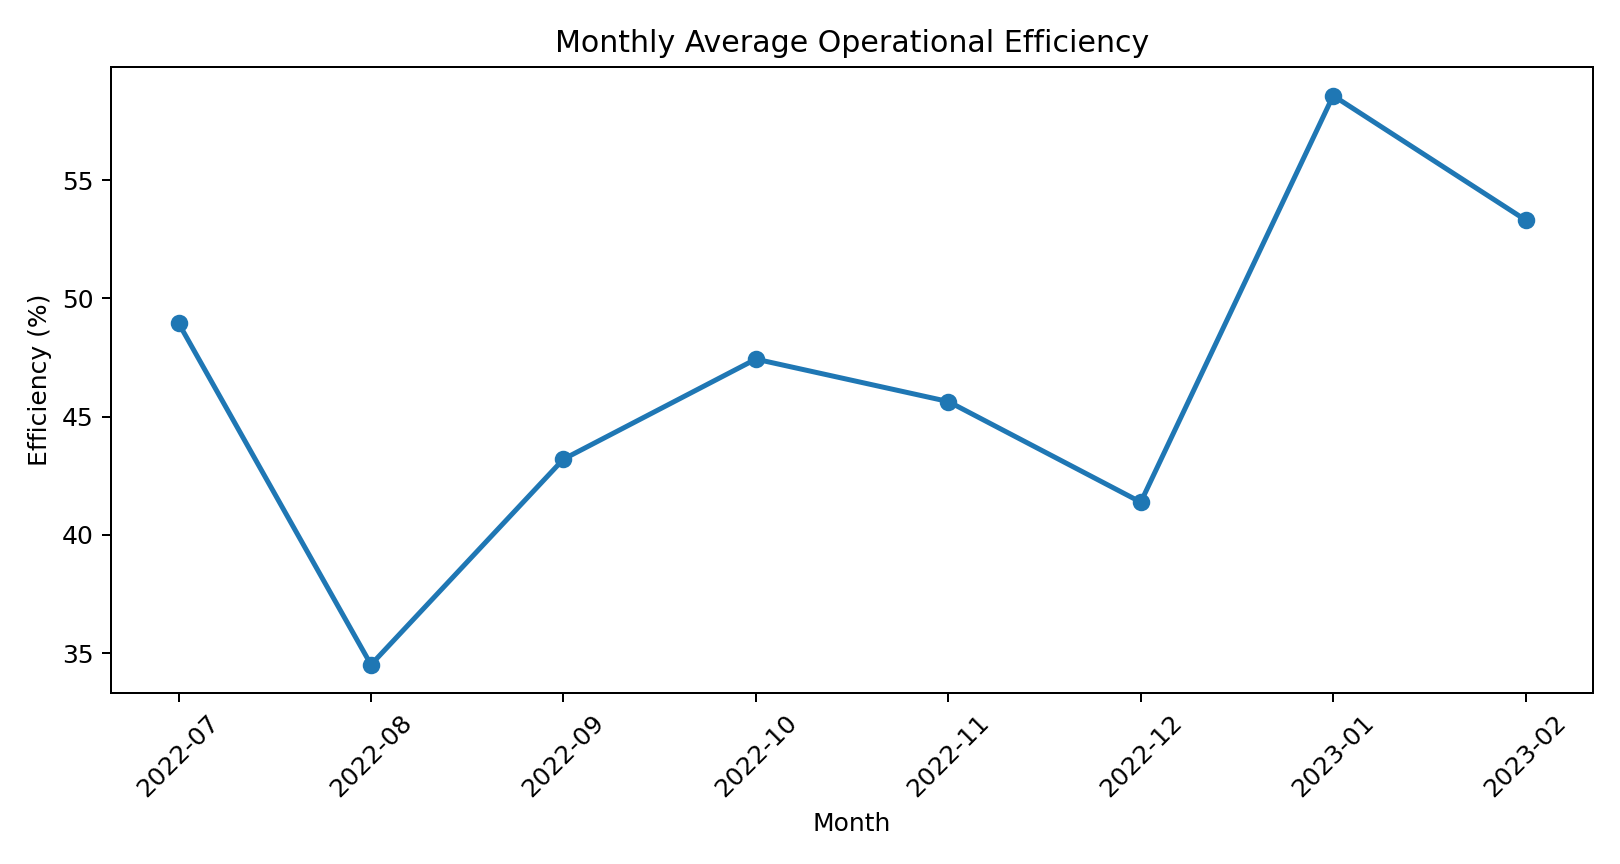
\includegraphics[width=0.9\textwidth]{outputs/monthly_efficiency.png}
\caption{Monthly average operational efficiency from the real dataset.}
\end{figure}

\subsection{Downtime Structure}
The downtime-event distribution is strongly right-skewed. The median event duration is 1.50 min, the 90th percentile is 6.50 min, the 95th percentile is 13.74 min, and the maximum observed event is 349.83 min.

\begin{table}[H]
\centering
\caption{Downtime Category Structure}
\begin{tabular}{lrr}
\toprule
Category & Event Count & Share of Downtime Minutes \\
\midrule
Micro ($\leq$ 2 min) & 851 & 13.59\% \\
Minor (2--10 min) & 443 & 20.15\% \\
Major ($>$ 10 min) & 94 & 66.26\% \\
\bottomrule
\end{tabular}
\end{table}

\begin{figure}[H]
\centering
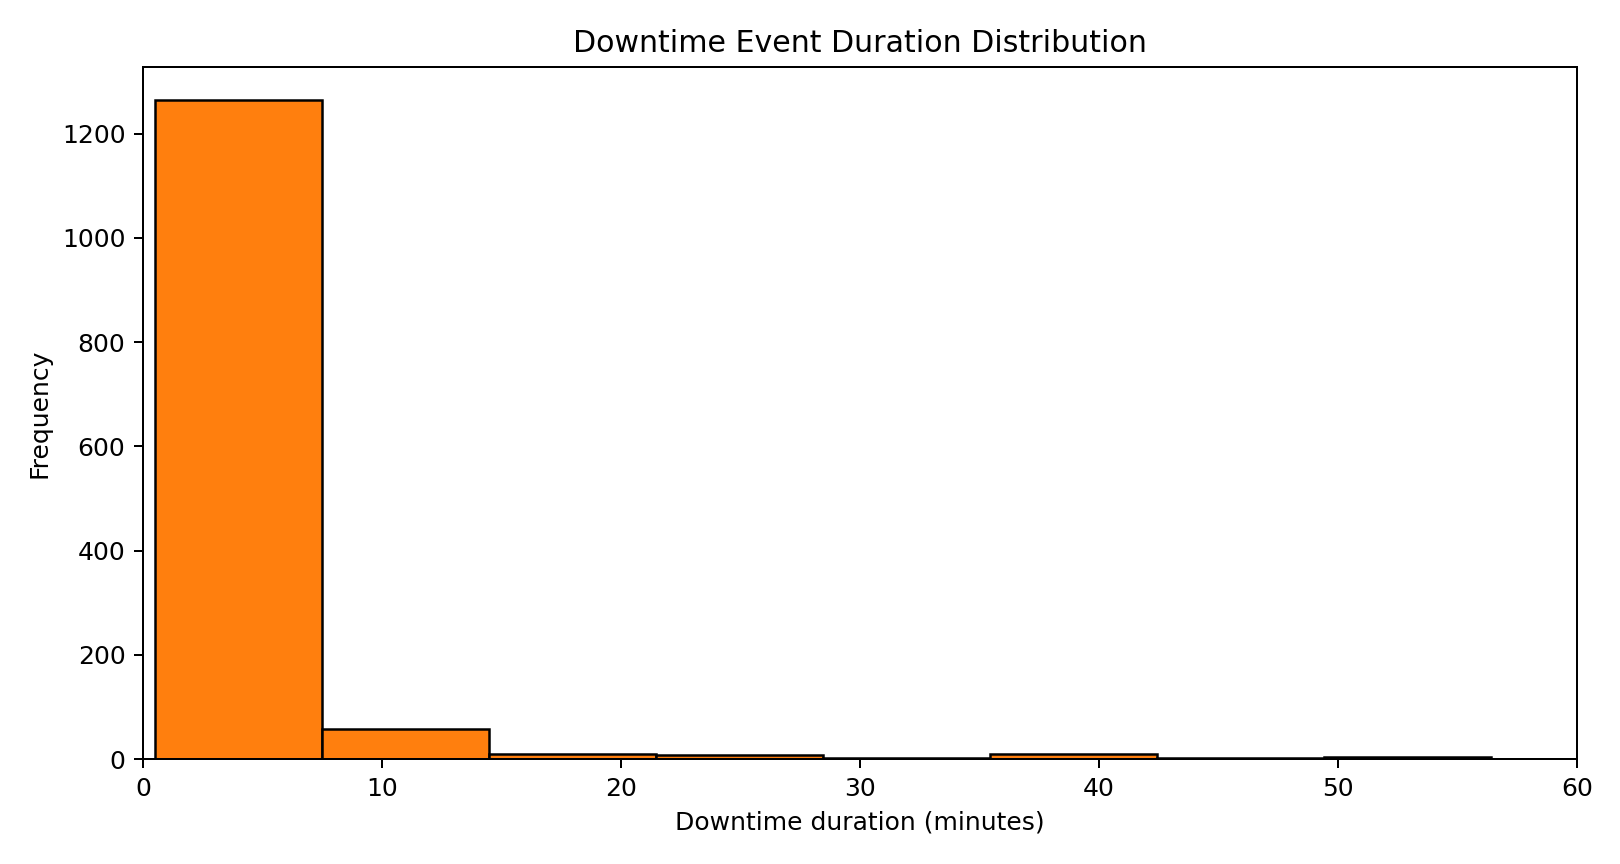
\includegraphics[width=0.9\textwidth]{outputs/downtime_distribution.png}
\caption{Distribution of downtime-event duration, truncated at 60 minutes for readability.}
\end{figure}

\begin{figure}[H]
\centering
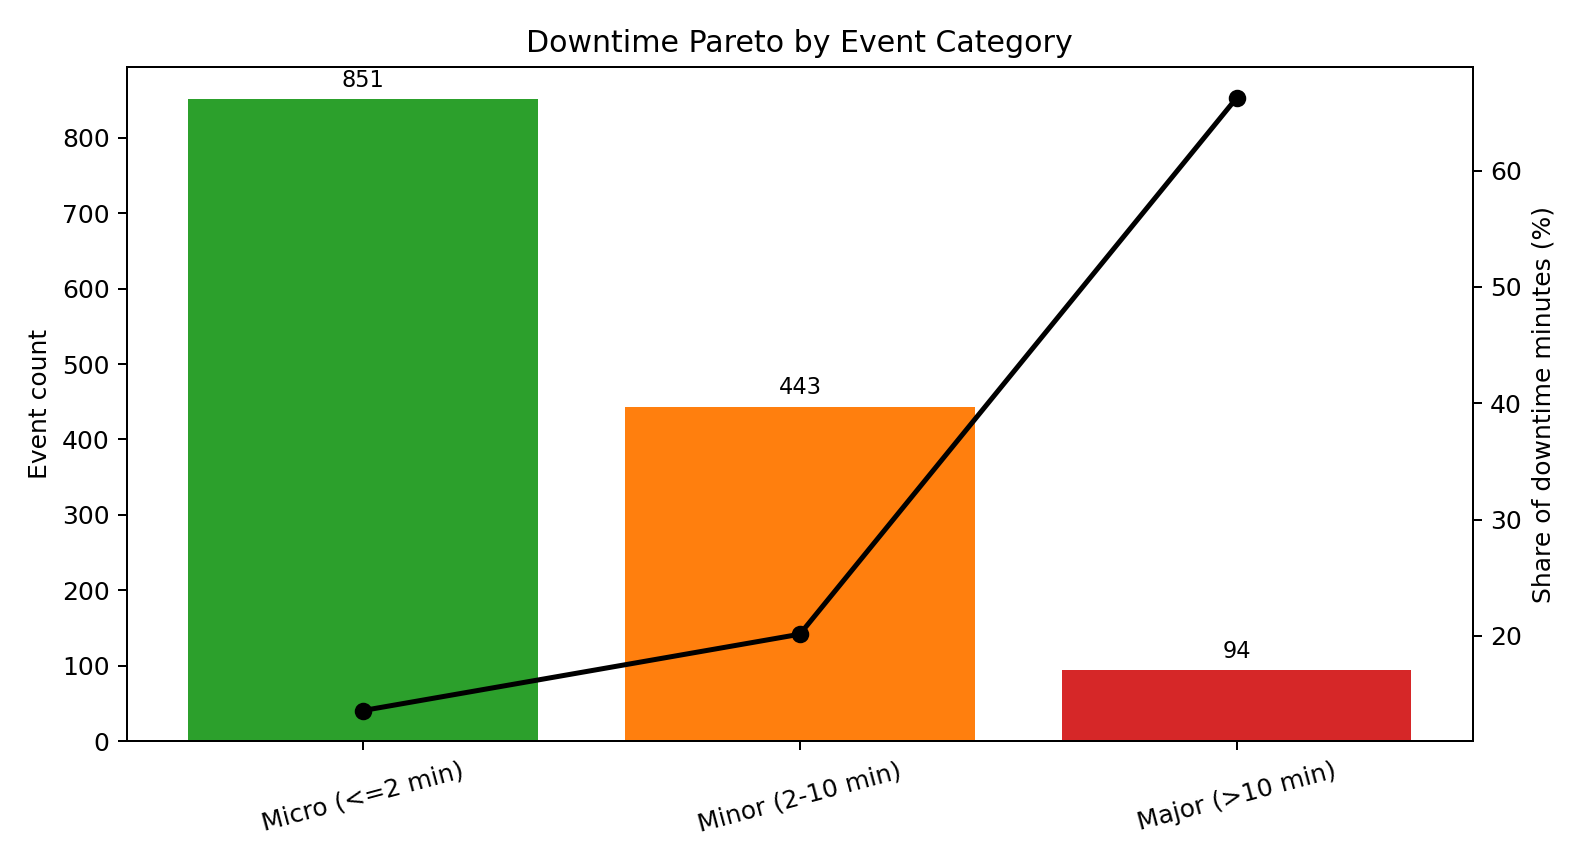
\includegraphics[width=0.9\textwidth]{outputs/downtime_category_pareto.png}
\caption{Downtime Pareto by event category.}
\end{figure}

Micro-stoppages account for 61.31\% of all events but only 13.59\% of total downtime minutes, whereas major stoppages account for 6.77\% of events but consume 66.26\% of lost time. This is the central explanation for why maintenance-focused interventions outperform purely organizational interventions.

\begin{figure}[H]
\centering
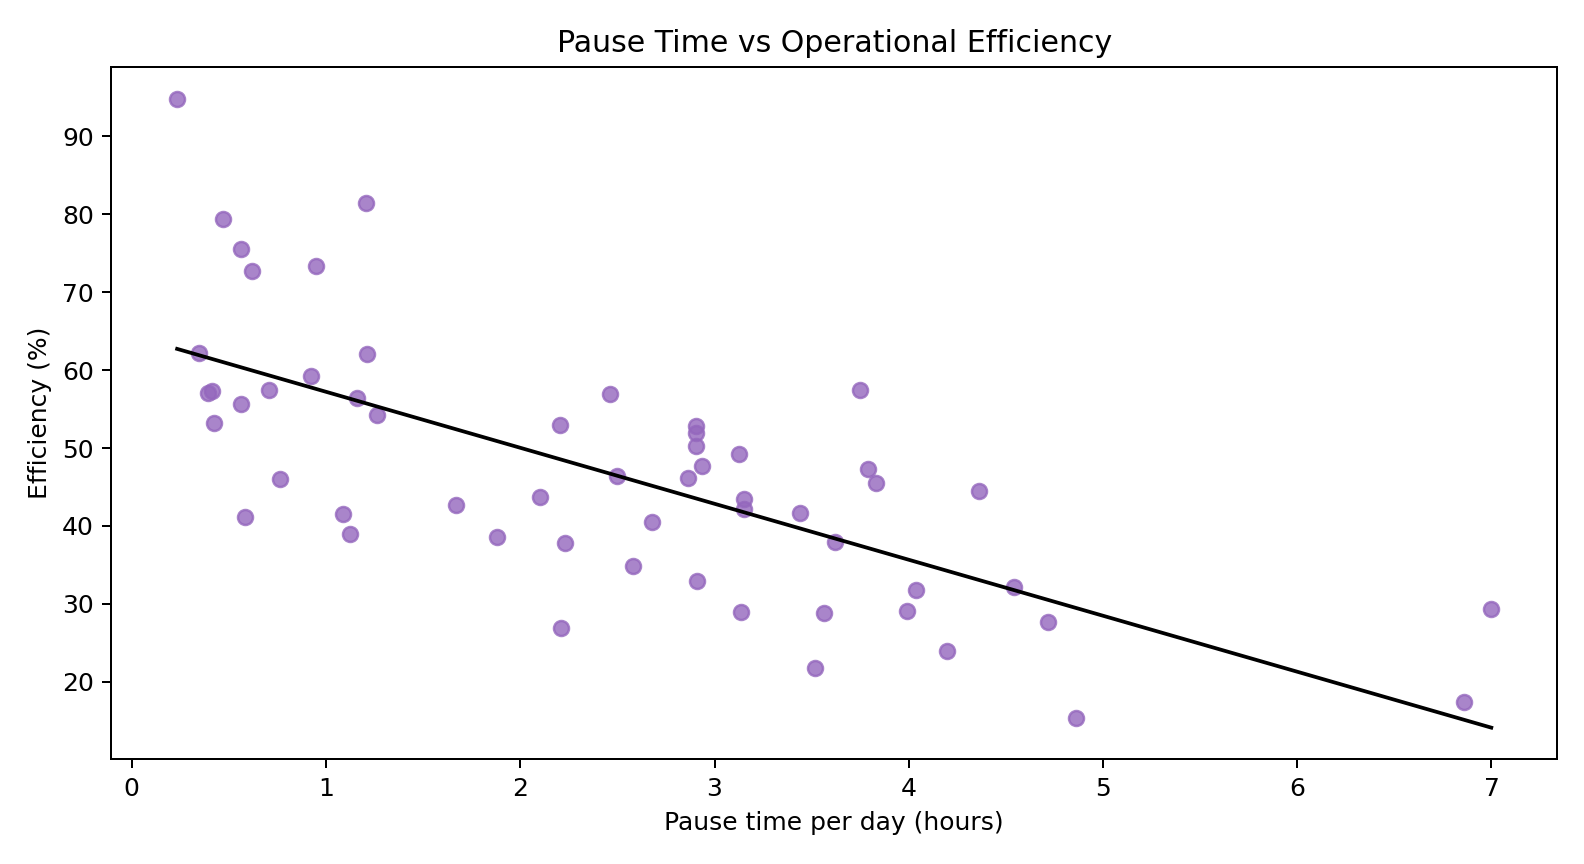
\includegraphics[width=0.9\textwidth]{outputs/pause_vs_efficiency.png}
\caption{Daily pause time versus operational efficiency.}
\end{figure}

\subsection{Scenario Results}
The simulation baseline produced 211,924.69 liters on average across the resampled production horizon, closely matching the observed system output.

\begin{table}[H]
\centering
\caption{Simulation Results for Lean Scenarios}
\begin{tabular}{lrrrr}
\toprule
Scenario & Output (L) & Gain (\%) & Efficiency (\%) & Gain (pp) \\
\midrule
Baseline & 211,924.69 & 0.00 & 42.37 & 0.00 \\
5S + Visual Mgmt. & 216,866.69 & 2.33 & 43.25 & 0.88 \\
TPM & 255,604.10 & 20.61 & 50.81 & 8.44 \\
Integrated Bundle & 280,142.22 & 32.19 & 55.33 & 12.96 \\
\bottomrule
\end{tabular}
\end{table}

\begin{figure}[H]
\centering
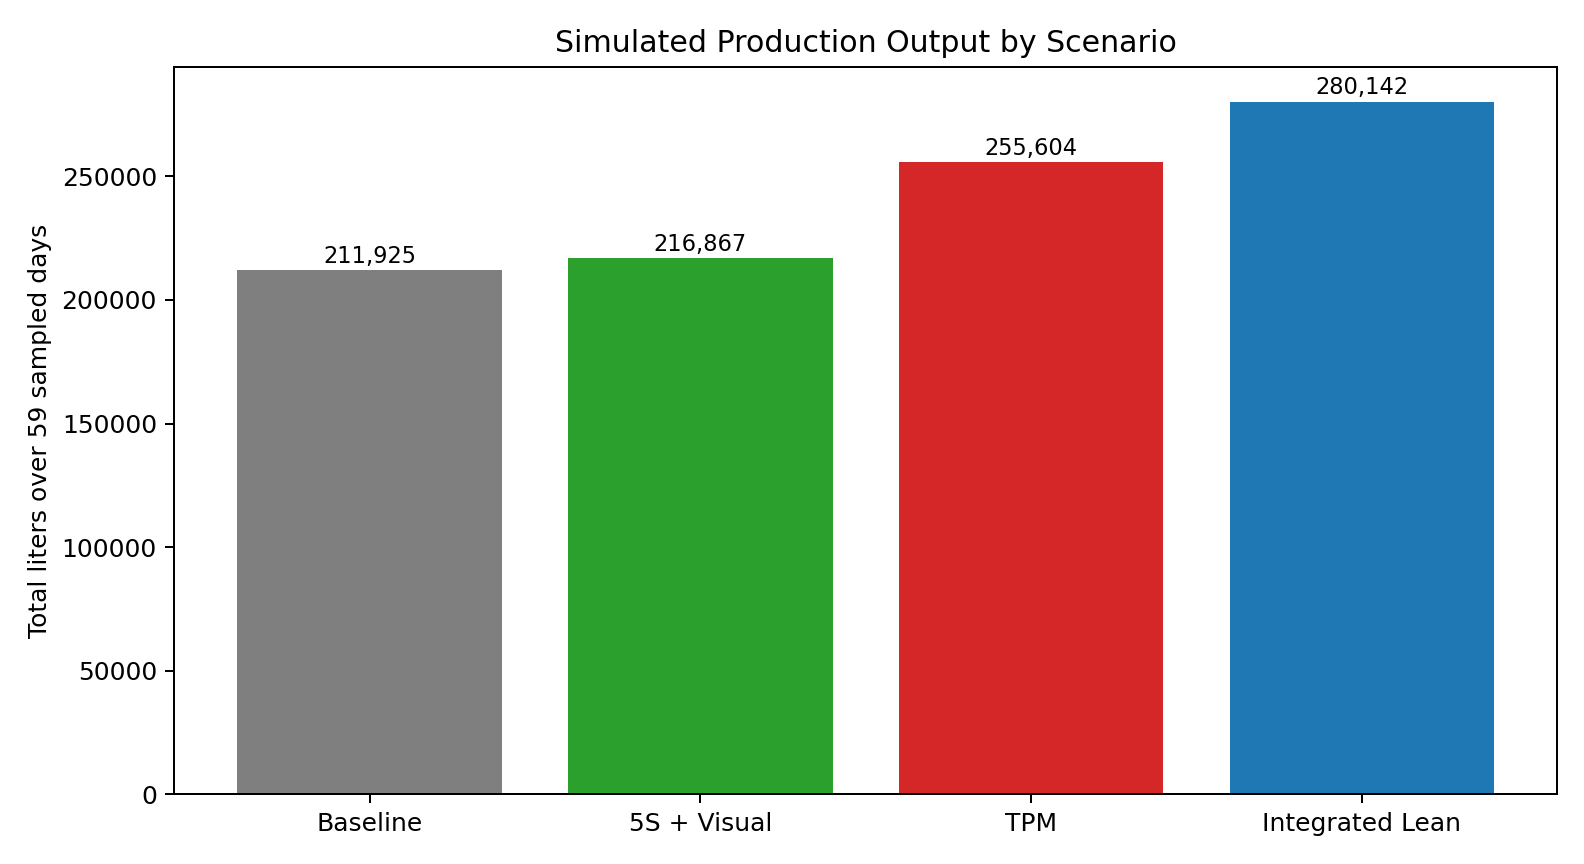
\includegraphics[width=0.9\textwidth]{outputs/scenario_output.png}
\caption{Mean simulated output across the baseline and lean scenarios.}
\end{figure}

The 5S scenario produces only a modest gain because it mainly targets frequent but short stoppages. TPM produces a much larger improvement because it directly attacks the dominant lost-time source. The integrated lean bundle produces the best result because it reduces losses across all stoppage categories.

\section{Discussion}
The results show that lean implementation should be based on the structure of loss rather than the visibility of events. In many production systems, micro-stoppages attract attention because they occur frequently, but they may not be the dominant source of lost output. In the present case, major stoppages are relatively rare but consume most of the downtime minutes, which makes TPM the highest-priority intervention.

This finding is aligned with earlier lean-simulation work showing that the effect of lean tools depends on system context [4], [5]. It also supports the broader argument that simulation is particularly useful for SMEs because it reduces the risk of poor implementation sequencing [3].

The study also strengthens the connection between lean and digital manufacturing. Instead of relying only on static value stream maps or qualitative observation, the analysis uses real event-level data, operational variability, and scenario simulation. This is consistent with the direction suggested by smart manufacturing and digital twin literature [6], [10].

\section{Conclusion}
This paper presented a journal-style, self-contained study on simulation-based lean manufacturing using a real industrial beverage bottling dataset. The line suffers from low availability, high downtime, and significant variability over time. Although micro-stoppages are the most frequent events, major stoppages dominate total lost time.

The simulation showed that 5S and visual management improve output by 2.33\%, total productive maintenance improves output by 20.61\%, and an integrated lean bundle improves output by 32.19\% while increasing simulated availability from 42.37\% to 55.33\%.

The main practical implication is that maintenance-led reduction of major stoppages should be prioritized first, followed by workplace organization and broader line stabilization. The main academic contribution is a reproducible open-data framework for lean-simulation research suitable for final-year engineering projects and SME-oriented manufacturing analysis.

\section*{Acknowledgment}
The authors sincerely acknowledge the guidance and support of Dr.\ MOHD SHUAIB from the Mechanical Department. His academic guidance was valuable in shaping the direction and structure of this work.

\begin{thebibliography}{11}

\bibitem{r1}
I. Belekoukias, J. A. Garza-Reyes, and V. Kumar, ``The impact of lean methods and tools on the operational performance of manufacturing organisations,'' \emph{International Journal of Production Research}, vol. 52, no. 18, pp. 5346--5366, 2014, doi: 10.1080/00207543.2014.903348.

\bibitem{r2}
O. Oleghe and K. Salonitis, ``Hybrid simulation modelling of the human-production process interface in lean manufacturing systems,'' \emph{International Journal of Lean Six Sigma}, vol. 10, no. 2, pp. 665--690, 2019, doi: 10.1108/IJLSS-01-2018-0004.

\bibitem{r3}
F. Yu and Z. Chen, ``Tools, application areas and challenges of factory simulation in Small and Medium-Sized Enterprises -- A Review,'' \emph{Procedia CIRP}, vol. 104, pp. 399--404, 2021, doi: 10.1016/j.procir.2021.11.067.

\bibitem{r4}
J. Possik, A. Zouggar-Amrani, B. Vallespir, and G. Zacharewicz, ``Lean techniques impact evaluation methodology based on a co-simulation framework for manufacturing systems,'' \emph{International Journal of Computer Integrated Manufacturing}, vol. 35, no. 1, pp. 91--111, 2022, doi: 10.1080/0951192X.2021.1972468.

\bibitem{r5}
S. Frecassetti, B. Kassem, K. Kundu, M. Ferrazzi, and A. Portioli-Staudacher, ``Introducing Lean practices through simulation: A case study in an Italian SME,'' \emph{Quality Management Journal}, vol. 30, no. 2, pp. 90--104, 2023, doi: 10.1080/10686967.2023.2171326.

\bibitem{r6}
J. A. C. Bokhorst, W. Knol, J. Slomp, and T. Bortolotti, ``Assessing to what extent smart manufacturing builds on lean principles,'' \emph{International Journal of Production Economics}, vol. 253, art. no. 108599, 2022, doi: 10.1016/j.ijpe.2022.108599.

\bibitem{r7}
G. A. David, P. M. C. Monson, C. Soares Junior, P. O. Conceicao Junior, P. R. Aguiar, and A. Simeone, ``IoT-Driven Deep Learning for Enhanced Industrial Production Forecasting,'' \emph{IEEE Internet of Things Journal}, vol. 11, no. 23, pp. 38486--38495, 2024, doi: 10.1109/JIOT.2024.3447579.

\bibitem{r8}
G. A. David, P. M. C. Monson, and C. Soares Junior, \emph{Industrial Production Time-Series Dataset from a Beverage Bottling Line}. Zenodo, Jan. 4, 2026. doi: 10.5281/zenodo.18146866.

\bibitem{r9}
J. M. Matindana and M. J. Shoshiwa, ``Lean manufacturing implementation in food and beverage SMEs in Tanzania: using structural equation modelling (SEM),'' \emph{Management System Engineering}, vol. 4, no. 1, pp. 1--14, 2025, doi: 10.1007/s44176-025-00036-3.

\bibitem{r10}
M. Reslan, M. J. Triebe, R. Venketesh, and A. J. Hartwell, ``Automation of Value Stream Mapping: A Case Study on Enhancing Lean Manufacturing Tools Through Digital Twins,'' \emph{Procedia CIRP}, vol. 134, pp. 455--460, 2025, doi: 10.1016/j.procir.2025.02.159.

\bibitem{r11}
C. Unal and S. Bilget, ``Examination of lean manufacturing systems by simulation technique in apparel industry,'' \emph{The Journal of The Textile Institute}, vol. 112, no. 3, pp. 377--387, 2021, doi: 10.1080/00405000.2020.1756104.

\end{thebibliography}

\end{document}
